\documentclass[aspectratio=169,11pt]{beamer}
\usetheme{Madrid}
\usecolortheme{default}
\setbeamertemplate{navigation symbols}{}
\usepackage{amsmath,amssymb}
\usepackage{booktabs}
\usepackage{graphicx}
\usepackage{tikz}
\usepackage{xcolor}

\title[ML Prediction of Band Gap]{Machine Learning-Based Prediction of Semiconductor Band Gap}
\subtitle{Physics-Informed Materials Descriptors and 3D structure analysis}
\vspace{4in}
\author{Muhammad Fayaz}
\vspace{5in}
\institute{Department of Physics \\
(uop)}
\vspace{3in}
\date{\today}

\begin{document}

\begin{frame}
  \titlepage
\end{frame}

\begin{frame}{Presentation Outline}
\tableofcontents
\end{frame}

\section{Background}

\begin{frame}{Understanding the Semiconductor Band Gap}
	
	\begin{columns}[T]
		
		%==================================================
		% LEFT COLUMN
		%==================================================
		\begin{column}{0.6\textwidth}
			
			\begin{block}{What is the Band Gap?}
				The band gap $E_g$ is the energy separation between
				the valence-band maximum and conduction-band minimum.
			\end{block}
			
%			\vspace{0.1cm}
			
			\begin{itemize}
				\item It strongly influences electrical transport
				and optical absorption.
				\item A photon can promote an electron across the
				gap when
				\[
				h\nu \geq E_g.
				\]
				\item Band-gap engineering is important for
				photovoltaics, LEDs, photodetectors and
				other optoelectronic devices.
			\end{itemize}
			
%			\vspace{0.1cm}
			
		
			
		\end{column}
		
		
		%==================================================
		% RIGHT COLUMN
		%==================================================
		\begin{column}{0.4\textwidth}
			
			\begin{center}
				
%				\includegraphics[
%				width=0.60\linewidth
%				]{bandgap_concept.png}
				
				\vspace{0.15cm}
				
				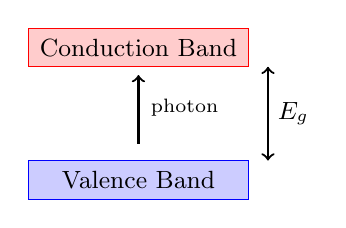
\begin{tikzpicture}[scale=0.70]
				
				% Valence band
				\draw[fill=blue!20, draw=blue]
				(0,0) rectangle (4,0.7);
				
				\node at (2,0.35)
				{\small Valence Band};
				
				% Conduction band
				\draw[fill=red!20, draw=red]
				(0,2.4) rectangle (4,3.1);
				
				\node at (2,2.75)
				{\small Conduction Band};
				
				% Band gap arrow
				\draw[<->, thick]
				(4.35,0.7) -- (4.35,2.4);
				
				\node[right] at (4.35,1.55)
				{\small $E_g$};
				
				% Electron excitation arrow
				\draw[->, thick]
				(2,1.0) -- (2,2.25);
				
				\node[right] at (2.05,1.65)
				{\scriptsize photon};
				
				\end{tikzpicture}
				
				\vspace{0.1cm}
				
				\small
				\textit{Electronic excitation across the band gap}
					\begin{alertblock}{Key Relationship}
					\centering
					\[
					\boxed{h\nu \geq E_g}
					\]
					Photon energy must be sufficient to excite
					an electron across the band gap.
				\end{alertblock}
			\end{center}
			
		\end{column}
		
	\end{columns}
	
\end{frame}

\begin{frame}{Why Predict Band Gap from Composition?}
\begin{itemize}
  \item Experimental band-gap determination can require synthesis and characterization.
  \vspace{1cm}
  \item Chemical composition contains information about atomic mass, atomic number and electronegativity.
  \vspace{1cm}
  \item Machine learning can learn nonlinear relationships between composition-derived descriptors and measured band gaps.
  \vspace{1cm}
  \item The project therefore connects \textbf{materials physics + descriptors + machine learning}.
\end{itemize}
\end{frame}

\begin{frame}{Band Gap and Optical Absorption}
	
	\begin{columns}[c]
		
		% Left column
		\begin{column}{0.48\textwidth}
			
			\begin{block}{Absorption-Edge Relation}
				For a simplified absorption-edge estimate:
				\[
				\lambda_{\mathrm{edge}}
				\approx
				\frac{1240}{E_g}\;\text{nm},
				\]
				where $E_g$ is the band gap in eV.
			\end{block}
			
			\vspace{0.25cm}
			
			\begin{itemize}
				\item Larger $E_g$
				$\Rightarrow$ shorter-wavelength edge.
				
				\item Smaller $E_g$
				$\Rightarrow$ longer-wavelength edge.
			\end{itemize}
			
		\end{column}
		
		% Right column
		\begin{column}{0.48\textwidth}
			
			\begin{block}{Example}
				A predicted band gap of
				\[
				E_g = 2.570\;\text{eV}
				\]
				gives
				\[
				\lambda_{\mathrm{edge}}
				\approx
				\frac{1240}{2.570}
				= 482.490\;\text{nm}.
				\]
				
				\vspace{0.15cm}
				
				This wavelength lies in the
				\textbf{visible region}.
			\end{block}
			
			\vspace{0.2cm}
			
			\begin{alertblock}{Important Note}
				This is an approximate conversion and
				not a complete optical-property model.
			\end{alertblock}
			
		\end{column}
		
	\end{columns}
	
\end{frame}

\section{Dataset and Features}

\begin{frame}{Dataset Used in the Project}
	
	\begin{columns}[c]
		
		% Left column
		\begin{column}{0.48\textwidth}
			\begin{block}{Dataset Overview}
				\begin{itemize}
					\item \textbf{Dataset:} \texttt{matbench\_expt\_gap}
					\item \textbf{Samples:} 4,604 materials
					\item \textbf{Input:} Chemical composition
					\item \textbf{Target:} Experimental band gap (eV)
				\end{itemize}
			\end{block}
			
			\vspace{0.3cm}
			
			\begin{alertblock}{Data Preparation}
				4,604 materials remained after the
				loading and cleaning steps.
			\end{alertblock}
		\end{column}
		
		% Right column
		\begin{column}{0.48\textwidth}
			\begin{center}
				\includegraphics[
				width=0.95\linewidth
				]{bandgap_distribution.png}
				
				\vspace{0.15cm}
				
				\small
				\textit{Distribution of experimental band gaps}
			\end{center}
		\end{column}
		
	\end{columns}
	
\end{frame}

\begin{frame}{Physics-Informed Composition Features}
	
	\begin{columns}[c]
		
		% Left column
		\begin{column}{0.48\textwidth}
			
			\begin{block}{Structural Features}
				\begin{itemize}
					\item Number of elements
					\item Total atoms in reduced formula
				\end{itemize}
			\end{block}
			
			\vspace{0.15cm}
			
			\begin{block}{Atomic Properties}
				\begin{itemize}
					\item Average atomic mass
					\item Maximum atomic number
					\item Minimum atomic number
				\end{itemize}
			\end{block}
			
		\end{column}
		
		% Right column
		\begin{column}{0.48\textwidth}
			
			\begin{block}{Electronegativity Features}
				\begin{itemize}
					\item Maximum electronegativity
					\item Minimum electronegativity
					\item Electronegativity difference
				\end{itemize}
			\end{block}
			
			\vspace{0.25cm}
			
			\begin{alertblock}{Why These Features?}
				They convert chemical composition into a
				compact numerical representation that can
				be directly used by regression models.
			\end{alertblock}
			
		\end{column}
		
	\end{columns}
	
	\vspace{0.25cm}
	
	\begin{center}
		\small
		\textit{Composition}
		$\quad\longrightarrow\quad$
		\textit{Physics-informed descriptors}
		$\quad\longrightarrow\quad$
		\textit{Band-gap prediction}
	\end{center}
	
\end{frame}
\begin{frame}{Experimental Band-Gap Categories}
	
	\begin{columns}[c]
		
		% Left column
		\begin{column}{0.48\textwidth}
			\textbf{The notebook groups materials as:}
			
			\vspace{0.3cm}
			
			\begin{itemize}
				\item \textbf{Low band gap:}
				$E_g < 1.0$ eV
				
				\vspace{0.15cm}
				
				\item \textbf{Intermediate band gap:}
				$1.0 \leq E_g < 3.0$ eV
				
				\vspace{0.15cm}
				
				\item \textbf{Wide band gap:}
				$E_g \geq 3.0$ eV
			\end{itemize}
		\end{column}
		
		% Right column
		\begin{column}{0.55\textwidth}
			\begin{center}
				\includegraphics[width=\linewidth]{bandgap_categories.png}
			\end{center}
		\end{column}
		
	\end{columns}
	
\end{frame}
\section{Machine Learning Methodology}

%\begin{frame}{Machine Learning Workflow}
%\begin{center}
%\begin{tikzpicture}[node distance=0.75cm, every node/.style={font=\small},
%box/.style={draw, rounded corners, align=center, minimum width=2.5cm, minimum height=0.8cm}]
%\node[box] (data) {Experimental\\band-gap data};
%\node[box, right=of data] (feat) {Composition\\features};
%\node[box, right=of feat] (split) {Train/Test\\split};
%\node[box, below=of split] (scale) {Feature\\standardization};
%\node[box, left=of scale] (models) {Regression\\models};
%\node[box, left=of models] (eval) {MAE, RMSE\\and $R^2$};
%\draw[->] (data)--(feat);
%\draw[->] (feat)--(split);
%\draw[->] (split)--(scale);
%\draw[->] (scale)--(models);
%\draw[->] (models)--(eval);
%\end{tikzpicture}
%\end{center}
%\end{frame}

\begin{frame}{Models Evaluated}
\begin{enumerate}
  \item Linear Regression
  \item Random Forest Regression
  \item Gradient Boosting Regression
  \item Deep Neural Network
\end{enumerate}

\begin{block}{Data split}
The notebook uses an 80/20 train--test split with \texttt{random\_state=42}.
\end{block}

\begin{block}{Deep network}
The implemented network uses dense layers of 128, 64 and 32 units, batch normalization, dropout and a linear output for continuous band-gap prediction.
\end{block}
\end{frame}

\section{Results}

\begin{frame}{Model Performance}
\begin{center}
\includegraphics[width=0.95\linewidth]{model_metrics.png}
\end{center}
\end{frame}

\begin{frame}{Model Performance: Numerical Results}
\small
\begin{tabular}{lccc}
\toprule
Model & MAE (eV) & RMSE (eV) & $R^2$\\
\midrule
Linear Regression & 0.997824 & 1.326643 & 0.181688\\
Random Forest & 0.518957 & 0.904775 & 0.619380\\
Gradient Boosting & 0.669760 & 1.020542 & 0.515747\\
Deep Neural Network & 0.698311 & 1.090020 & 0.447568\\
\bottomrule
\end{tabular}

\vspace{0.5cm}
\begin{itemize}
  \item In the notebook's MAE-based selection, Random Forest is selected as the model used for the subsequent actual-vs-predicted and error plots.
\end{itemize}
\end{frame}

\begin{frame}{Actual vs Predicted Band Gap}
	
	\begin{columns}[c]
		
		% Left column
		\begin{column}{0.4\textwidth}
			\begin{center}
				\includegraphics[
				width=\linewidth
				]{actual_vs_predicted.png}
			\end{center}
		\end{column}
		
		% Right column
		\begin{column}{0.45\textwidth}
			
			\begin{block}{Model Agreement}
				The plot compares the experimental
				band-gap values with the values
				predicted by the regression model.
			\end{block}
			
			\vspace{0.18cm}
			
			\begin{alertblock}{Ideal Prediction}
				The dashed diagonal line represents
				ideal agreement:
				\[
				E_g^{\mathrm{pred}}
				=
				E_g^{\mathrm{actual}}.
				\]
			\end{alertblock}
			
			\vspace{0.15cm}
			
			\small
			Points closer to the diagonal indicate
			closer agreement between experimental
			and predicted band-gap values.
			
		\end{column}
		
	\end{columns}
	
\end{frame}

\begin{frame}{Prediction Error Distribution}
\begin{center}
\includegraphics[width=0.58\linewidth]{prediction_error.png}
\end{center}
\small
Prediction error is defined in the notebook as predicted band gap minus experimental band gap.
\end{frame}

\begin{frame}{Deep Neural Network Training}
\begin{center}
\includegraphics[width=0.58\linewidth]{dnn_training.png}
\end{center}
\small
Training and validation loss curves are used to inspect learning behavior during training.
\end{frame}

\begin{frame}{Feature Importance}
\begin{center}
\includegraphics[width=0.78\linewidth]{feature_importance.png}
\end{center}
\end{frame}

\section{Materials Analysis}

\begin{frame}{Example: TiO$_2$ Prediction}
%The notebook contains a new-material prediction example for TiO$_2$.
\begin{block}{Recorded notebook result}
Predicted band gap for TiO$_2$: \textbf{2.510 eV}.
\end{block}

A separate optical-analysis example in the notebook reports:
\[
E_g=2.570~\mathrm{eV},\qquad
\lambda_{\mathrm{edge}}\approx494~\mathrm{nm}.
\]

\begin{itemize}
  \item These outputs illustrate how a predicted band gap can be connected to a simple optical-edge estimate.
\end{itemize}
\end{frame}

\begin{frame}{Example: GaAs Complete Analysis}
The notebook's complete material-analysis example reports:
\begin{itemize}
  \item Composition: GaAs
  
  \item Number of elements: 2
  
  \item Predicted band gap: $1.008$ eV
  
  \item Estimated absorption edge: $873.24$ nm
  
  \item Spectral region: Near Infrared (NIR)
\end{itemize}
\end{frame}

\section{Discussion and Conclusion}

\begin{frame}{Key Findings}
\begin{itemize}
  \item The project demonstrates an end-to-end workflow from experimental composition--band-gap data to machine-learning prediction.
  \item Composition-derived physics-inspired descriptors can be used as model inputs.
  \item Four regression approaches were evaluated.
  \item The recorded test-set metrics show different levels of predictive performance across the models.
  \item The notebook uses Random Forest for the subsequent best-model visualization based on the lowest MAE.
\end{itemize}
\end{frame}

%\begin{frame}{Future Work}
%\begin{itemize}
%%  \item Composition-only descriptors do not explicitly encode crystal structure, defects, strain or measurement conditions.
%%  \item Experimental band gaps may be affected by measurement method and material quality.
%  \item Future work can incorporate crystal-structure descriptors, formation-energy-related features and uncertainty estimation.
%  \vspace{1cm}
%  \item External validation on a held-out materials family would strengthen assessment of generalization.
%\end{itemize}
%\end{frame}

\begin{frame}{Live Streamlit Application: Band-Gap Prediction} 
	\begin{columns}[T]  
\begin{column}{0.52\textwidth} \textbf{Interactive Machine Learning Platform} 
%			\begin{itemize} \item A live \textbf{Streamlit web application} was developed for real-time band-gap prediction. \item Users can enter or select material composition and obtain an estimated semiconductor band gap. \item The application provides an interactive interface for demonstrating the trained ML model. \item Predictions can be connected directly to the trained \textbf{Random Forest regression model}. \item The platform provides a practical demonstration of the proposed materials-informatics workflow. \end{itemize} 
			\vspace{0.2cm} \textbf{Local deployment:} 
		\begin{center} \Large \texttt{http://localhost:8501} \end{center} 
	\end{column}
		  \begin{column}{0.44\textwidth} 
%		 	 	\begin{block} \centering \Large \textbf{Streamlit App}\\[0.25cm] \texttt{localhost:8501}\\[0.35cm] \small Composition $\rightarrow$ Features $\rightarrow$ ML Model $\rightarrow$ Predicted Band Gap 
%		 	\end{block} \vspace{0.3cm} 
%	 	\begin{alertblock}{Application Goal} Demonstrate how the trained machine-learning model can be used interactively for rapid screening of semiconductor materials. \end{alertblock} 
 	\end{column} 
 \end{columns} 
\end{frame}
\begin{frame}{Conclusion}
\begin{itemize}
  \item Machine learning provides a practical route for rapid screening of materials by estimated band gap.
  \item The project combines fundamental semiconductor physics with materials informatics.
  \item The workflow can be extended toward candidate screening for photovoltaic and optoelectronic materials.
\end{itemize}

\vfill
\begin{center}
\Large Thank You
\end{center}
\end{frame}

\end{document}